\documentclass[a4paper, 14pt]{extarticle}

% Поля
%--------------------------------------
\usepackage{geometry}
\geometry{a4paper,tmargin=2cm,bmargin=2cm,lmargin=3cm,rmargin=1cm}
%--------------------------------------


%Russian-specific packages
%--------------------------------------
\usepackage[T2A]{fontenc}
\usepackage[utf8]{inputenc}
\usepackage[english, main=russian]{babel}

%--------------------------------------

\usepackage{textcomp}

% Красная строка
%--------------------------------------
\usepackage{indentfirst}               
%--------------------------------------             


%Graphics
%--------------------------------------
\usepackage{graphicx}
\graphicspath{ {./images/} }
\usepackage{float}%"Плавающие" картинки
%--------------------------------------

% Полуторный интервал
%--------------------------------------
\linespread{1.3}                    
%--------------------------------------

%Выравнивание и переносы
%--------------------------------------
% Избавляемся от переполнений
\sloppy
% Запрещаем разрыв страницы после первой строки абзаца
\clubpenalty=10000
% Запрещаем разрыв страницы после последней строки абзаца
\widowpenalty=10000
%--------------------------------------

%Списки
\usepackage{enumitem}

%Подписи
\usepackage{caption} 

%Гиперссылки
% \usepackage{hyperref}

\usepackage[colorlinks, urlcolor = blue, filecolor = blue, citecolor = blue, linkcolor = black]{hyperref}


\hypersetup {
unicode=true
}

%Рисунки
%--------------------------------------
\DeclareCaptionLabelSeparator*{emdash}{~--- }
\captionsetup[figure]{labelsep=emdash,font=onehalfspacing,position=bottom}
%--------------------------------------

\usepackage{tempora}

% Листинг кода (требуется \texttt{pdflatex -shell-escape})
%--------------------------------------
\usepackage{minted}
%--------------------------------------

%%% Математические пакеты %%%
%--------------------------------------
\usepackage{amsthm,amsfonts,amsmath,amssymb,amscd}  % Математические дополнения от AMS
\usepackage{mathtools}                              % Добавляет окружение multlined
\usepackage[perpage]{footmisc}


% графики
\usepackage{booktabs}        % Пакет для улучшенных таблиц
\usepackage{longtable}      % Длинные таблицы на несколько страниц
\usepackage{pgfplots}        % Пакет для построения графиков
\pgfplotsset{compat=1.17}    % Установка совместимости
\usepackage{tikz}            % Пакет для создания диаграмм
\usetikzlibrary{arrows.meta, positioning, automata, decorations.pathreplacing, calc}

% Литература 

% переименовываем  список литературы в "список используемой литературы"
\addto\captionsrussian{\def\refname{Список литературы}}



\captionsetup[figure]{name=Рисунок, labelsep=space}

%--------------------------------------
\begin{document}

%--------------------------------------
%			ТИТУЛЬНЫЙ ЛИСТ
%--------------------------------------
\begin{titlepage}
\thispagestyle{empty}
\newpage

%Шапка титульного листа
%--------------------------------------
\vspace*{-60pt}
\hspace{-65pt}
\begin{minipage}{0.3\textwidth}
\hspace*{-20pt}\centering

\includegraphics[width=\textwidth]{emblem}
\end{minipage}
\begin{minipage}{0.67\textwidth}\small \textbf{
\vspace*{-0.7ex}
\hspace*{-6pt}\centerline{Министерство науки и высшего образования Российской Федерации}
\vspace*{-0.7ex}
\centerline{Федеральное государственное автономное образовательное учреждение }
\vspace*{-0.7ex}
\centerline{высшего образования}
\vspace*{-0.7ex}
\centerline{<<Московский государственный технический университет}
\vspace*{-0.7ex}
\centerline{имени Н.Э. Баумана}
\vspace*{-0.7ex}
\centerline{(национальный исследовательский университет)>>}
\vspace*{-0.7ex}
\centerline{(МГТУ им. Н.Э. Баумана)}}
\end{minipage}
%--------------------------------------

\vspace{-25pt}
\hspace{-35pt}\rule{\textwidth}{2.3pt}

\vspace*{-20.3pt}
\hspace{-35pt}\rule{\textwidth}{0.4pt}
%--------------------------------------

\vspace{1.5ex}
\hspace{-35pt} \noindent \small ФАКУЛЬТЕТ\hspace{80pt} <<Информатика и системы управления>>

\vspace*{-16pt}
\hspace{47pt}\rule{0.83\textwidth}{0.4pt}

\vspace{0.5ex}
\hspace{-35pt} \noindent \small КАФЕДРА\hspace{50pt} <<Теоретическая информатика и компьютерные технологии>>

\vspace*{-16pt}
\hspace{30pt}\rule{0.866\textwidth}{0.4pt}

\vspace{11em}

\begin{center}
\Large {\bf Домашнее задание №2} \\ 
\large <<Построение вероятностной модели (обобщённый парадокс Монти Холла)>> \\
\large {по курсу <<Моделирование>>} \\

\end{center}\normalsize

\vspace{8em}

\vbox{%
\hfill%
\vbox{%
\hbox{Студент: Аринин М.А.}%
\hbox{Группа: ИУ9-82Б}%
\hbox{Преподаватель: Домрачева А.Б.}%
}%
} 

\bigskip

\vfill

\begin{center}
\textsl{Москва 2026}
\end{center}
\end{titlepage}
%--------------------------------------

\setlength{\tabcolsep}{3pt}

\newpage
\setcounter{page}{2}

\section{Постановка задачи}

За одной из $N$ дверей находится приз, за остальными дверями пусто. Игрок выбирает одну дверь равновероятно. Ведущий, не открывая выбранную дверь и не открывая дверь с призом, открывает ровно $K$ пустых дверей (число $K$ удовлетворяет условию $1 \le K \le N-2$). После этого игрок с вероятностью $s$ сохраняет первоначальный выбор и с вероятностью $1-s$ меняет его, равновероятно выбирая одну из оставшихся закрытых дверей, отличную от текущего выбора.

\textbf{Цель работы:}
\begin{itemize}[nosep]
  \item описать эксперимент через введение событий $A$, $B$ и \textbf{формулу Байеса} для апостериорных вероятностей положения приза;
  \item по полученным вероятностям вывести $P(W)$ для стратегий «остаться», «сменить», смешанной стратегии с параметром $s$ и (при необходимости) байесовски оптимального решения на финальном шаге;
  \item реализовать модель программно и сопоставить теоретические вероятности с частотами метода Монте-Карло при разных значениях $s$ и разном числе прогонов $n$;
  \item для классического случая $N=3$, $K=1$ проверить согласованность симуляции с известными значениями парадокса Монти Холла;
  \item для $N=3,\ldots,10$ и $K=1,\ldots,N-2$ сравнить аналитику с Монте-Карло на полной сетке (в отчёте --- при $s=0{,}5$).
\end{itemize}

\textbf{Входные параметры модели:} $N$, $K$, вероятность сохранения выбора $s \in [0,1]$, число независимых прогонов симуляции $n$.

\textbf{Выходные данные:} теоретическая вероятность выигрыша (из байесовской модели и формул для стратегии), оценка по симуляции $\hat p$, величина $| \hat p - p_{\text{теор}} |$ и (при необходимости) расстояние между эмпирической и теоретической функциями распределения индикатора успеха на $\{0,1\}$.

\section{Построение математической модели}

\subsection{Формализация задачи}
Рассматривается \textbf{стохастическая (вероятностная) модель} дискретного случайного эксперимента. Основной аппарат --- \textbf{условные вероятности и формула Байеса}: по наблюдаемому действию ведущего (событию $B$) пересчитываются апостериорные вероятности положения приза, после чего для выбранной стратегии на завершающем этапе вычисляется $P(W)$.

Проверка адекватности программной реализации сводится к сравнению \textbf{частоты успеха} $\hat p$ в длинной серии независимых прогонов с теоретическим значением $p_{\text{теор}}$, полученным из той же байесовской постановки и формул стратегии (см.~\eqref{eq:mixed}). Дополнительно анализируется, как при росте $n$ уменьшается типичное отклонение $|\hat p - p_{\text{теор}}|$ и как меняются результаты при варьировании $s$.

\subsection{Предположения}
\begin{itemize}[nosep]
  \item приз равновероятно находится за любой из $N$ дверей;
  \item первый выбор игрока равновероятен;
  \item ведущий выбирает набор из $K$ открываемых пустых дверей равновероятно среди всех допустимых наборов (двери с призом и изначально выбранная игроком не открываются);
  \item при смене выбора игрок равновероятно берёт одну из закрытых дверей, отличных от текущей.
\end{itemize}

\subsection{Байесовская модель через события $A$ и $B$ и стратегия Трикса}
Введём события:
\begin{itemize}[nosep]
  \item $A$ --- приз находится за первоначально выбранной игроком дверью;
  \item $B$ --- ведущий открыл ровно $K$ пустых дверей, не открывая дверь с призом и текущий выбор игрока, и выбрал открываемые двери равновероятно среди всех допустимых наборов.
\end{itemize}
Априори $P(A)=1/N$, $P(\overline{A})=(N-1)/N$.

Если событие $A$ истинно, то среди остальных $N-1$ дверей все пусты и ведущий выбирает $K$ дверей из $N-1$ равновероятно, поэтому
\[
P(B\mid A)=\frac{1}{\mathrm{C}_{N-1}^{K}}.
\]
Если $A$ ложно, то среди остальных дверей есть одна дверь с призом, поэтому ведущий может выбирать только среди $N-2$ пустых дверей:
\[
P(B\mid \overline{A})=\frac{1}{\mathrm{C}_{N-2}^{K}}.
\]
Тогда по формуле Байеса получаем апостериорную вероятность того, что игрок угадал с первого раза:
\begin{equation}\label{eq:bayes_posterior}
P(A\mid B)=\frac{P(B\mid A)P(A)}{P(B\mid A)P(A)+P(B\mid \overline{A})P(\overline{A})}.
\end{equation}

После открытия $K$ пустых дверей остаётся $N-1-K$ альтернативных закрытых дверей (кроме текущей). По симметрии каждая из них имеет одинаковую апостериорную вероятность
\[
P(\text{приз за фиксированной альтернативной дверью}\mid B)=\frac{1-P(A\mid B)}{N-1-K}.
\]
Рациональная (байесовская) стратегия на финальном шаге --- выбрать дверь с большей апостериорной вероятностью. В частности, если
\[
\frac{1-P(A\mid B)}{N-1-K} > P(A\mid B),
\]
то выгодно \textbf{менять} выбор; иначе выгодно \textbf{оставаться}.

\textbf{Стратегия Трикса} --- это частный случай стратегии игрока: \textbf{всегда менять} выбор на финальном шаге. В обозначениях работы это соответствует $s=0$ и совпадает с «переключением» в классическом парадоксе Монти Холла.

\subsubsection{Вероятность выигрыша}
Обозначим через $W$ событие «игрок выиграл». При стратегии «всегда оставаться» ($s=1$) выигрыш тогда и только тогда, когда первый выбор совпал с призом:
\begin{equation}\label{eq:stay}
  P(W \mid \text{остаться}) = \frac{1}{N}.
\end{equation}

При стратегии «всегда менять» ($s=0$) разобьём по полной вероятности на случаи «первый выбор верный» и «первый выбор неверен». Если игрок сразу угадал приз (вероятность $1/N$), после открытия $K$ пустых среди остальных дверей все ещё закрытые альтернативы пусты, и смена ведёт к проигрышу. Если первый выбор неверен (вероятность $(N-1)/N$), приз находится среди $N-1$ остальных дверей; ведущий открывает $K$ пустых из них, остаётся $N-1-K$ закрытых «чужих» дверей, ровно одна из которых с призом. Игрок равновероятно выбирает одну из этих $N-1-K$ дверей, откуда
\begin{equation}\label{eq:switch}
  P(W \mid \text{сменить}) = \frac{N-1}{N} \cdot \frac{1}{N-1-K} = \frac{N-1}{N(N-1-K)}.
\end{equation}

Смешанная стратегия с вероятностью $s$ сохранить выбор даёт
\begin{equation}\label{eq:mixed}
  P(W) = s \cdot \frac{1}{N} + (1-s) \cdot \frac{N-1}{N(N-1-K)}.
\end{equation}

Классический парадокс Монти Холла соответствует $N=3$, $K=1$: $P(W\mid s=1)=1/3$, $P(W\mid s=0)=2/3$. Эти же значения получаются из~\eqref{eq:stay}--\eqref{eq:mixed} и согласуются с качественным выводом по апостериорным вероятностям после действия ведущего.

На рис.~\ref{fig:bayes_prob_tree} схематически показаны априорное ветвление по $A$ и $\overline{A}$, условные вероятности наблюдения $B$ в виде $1/\mathrm{C}_{N-1}^{K}$ и $1/\mathrm{C}_{N-2}^{K}$, формула Байеса и итоговые вероятности победы/поражения при чистых стратегиях; смешанная стратегия~\eqref{eq:mixed} --- выпуклая комбинация крайних случаев.

\begin{figure}[H]
\centering
\begin{tikzpicture}[
  font=\footnotesize,
  >=Stealth,
  node distance=0.55cm and 0.35cm,
  snode/.style={draw, rounded corners, align=center, inner sep=6pt},
  win/.style={draw, rounded corners, align=center, fill=green!14, inner sep=5pt},
  lose/.style={draw, rounded corners, align=center, fill=red!10, inner sep=5pt},
]
  \node[snode, minimum width=1.6cm] (S) {Старт};
  \node[snode, below left=1.15cm and 2.35cm of S] (A) {$A$:\\приз за изнач.\\выбором};
  \node[snode, below right=1.15cm and 2.35cm of S] (nA) {$\overline{A}$:\\приз не за\\изнач. выбором};
  \draw[->] (S) -- (A) node[pos=0.55, anchor=east, xshift=-6mm, font=\scriptsize] {$P(A)=\dfrac{1}{N}$};
  \draw[->] (S) -- (nA) node[pos=0.55, anchor=west, xshift=6mm, font=\scriptsize] {$P(\overline{A})=\dfrac{N-1}{N}$};

  \coordinate (midAn) at ($(A)!0.5!(nA)$);
  \node[snode, below=1.35cm of midAn, minimum width=4.2cm] (B) {$B$:\\ведущий открыл\\ровно $K$ пустых};
  \draw[->] (A) -- (B);
  \draw[->] (nA) -- (B);
  \coordinate (labA) at ($(A)!0.48!(B)$);
  \coordinate (labNA) at ($(nA)!0.48!(B)$);
  \node[anchor=east, xshift=-10mm, font=\scriptsize, align=right] at (labA) {$P(B\mid A)=\dfrac{1}{\mathrm{C}_{N-1}^{K}}$};
  \node[anchor=west, xshift=10mm, font=\scriptsize, align=left] at (labNA) {$P(B\mid\overline{A})=\dfrac{1}{\mathrm{C}_{N-2}^{K}}$};

  \node[snode, below=0.95cm of B, anchor=north, fill=yellow!12, text width=9.4cm] (bayes) {
    \textbf{Формула Байеса} (апостериор после наблюдения $B$):\\[0.35em]
    $\displaystyle P(A\mid B)=\frac{P(B\mid A)\,P(A)}{P(B\mid A)\,P(A)+P(B\mid\overline{A})\,P(\overline{A})}$
  };
  \draw[->, dashed] (B.south) -- ([yshift=2pt]bayes.north);

  \node[snode, below=1.0cm of bayes, text width=9.4cm, fill=blue!4] (finlab) {
    \textbf{Завершающий этап} (чистые стратегии): вероятности \textbf{победы} ($+$) и \textbf{поражения} ($-$) для одной партии
  };
  \draw[->, thick, darkgray] (bayes.south) -- (finlab.north);

  \node[win, below left=0.7cm and 0.1cm of finlab.south west, anchor=north east] (stayP) {Остаться:\\$P_{+}=1/N$};
  \node[lose, below=0.35cm of stayP] (stayM) {Остаться:\\$P_{-}=(N-1)/N$};

  \node[win, below right=0.7cm and 0.1cm of finlab.south east, anchor=north west] (swP) {Сменить:\\$P_{+}=\dfrac{N-1}{N(N-1-K)}$};
  \node[lose, below=0.35cm of swP] (swM) {Сменить:\\$P_{-}=1-\dfrac{N-1}{N(N-1-K)}$};

  \draw[->, thick, gray!70] (finlab.south) -- ++(0,-0.28) -- (stayP.north);
  \draw[->, thick, gray!70] (finlab.south) -- ++(0,-0.28) -- (swP.north);

  \node[below=0.45cm of stayM.south west, anchor=north west, font=\scriptsize, align=left, text width=9.2cm] (mixnote) {
  };
\end{tikzpicture}
\caption{Схема байесовской вероятностной модели: ветвление по $A$ и $\overline{A}$, наблюдение $B$, пересчёт $P(A\mid B)$, затем исходы победы/поражения при чистых стратегиях.}
\label{fig:bayes_prob_tree}
\end{figure}

\section{Решение вычислительных задач}

\subsection{Метод Монте-Карло}
Для фиксированных $N$, $K$, $s$ независимо моделируется большое число $n$ партий; оценка вероятности выигрыша --- выборочная доля $\hat p = (\text{число побед})/n$. Теоретическое значение $p_{\text{теор}}$ берётся из той же постановки, что и аналитика: для смешанной стратегии --- по~\eqref{eq:mixed}, для «всегда оставаться» и «всегда менять» --- как частные случаи.

\subsection{Согласование с классическим случаем}
Теоретические вероятности $p_{\text{теор}}$ для $N=3$, $K=1$ совпадают с~\eqref{eq:mixed} при $s=1$ и $s=0$ (то есть с $1/3$ и $2/3$). Симуляция сравнивается с этими значениями напрямую: $| \hat p - p_{\text{теор}} |$ и
\[
D_n = \sup_x |F_n(x) - F(x)| = |\hat p - p_{\text{теор}}|
\]
для индикатора успеха (ступенчатая $F$ на $\{0,1\}$). Величина $D_{\text{кр}} \approx k_{0{,}05}/\sqrt{n}$, $k_{0{,}05}=1{,}36$, взята из формулы Колмогорова для \emph{непрерывного} закона и для индикатора служит лишь грубым ориентиром по масштабу возможного отклонения при большом $n$ (буквальная интерпретация критерия здесь неприменима).

\subsection{Сеточный эксперимент по $(N,K)$}
Для каждой пары $(N,K)$ при фиксированном $s$ (в программе по умолчанию $s=0{,}5$) вычисляется $p_{\text{теор}}$ по~\eqref{eq:mixed} и оценка $\hat p$ по $n$ симуляциям.

\subsection{Варьирование $s$ и $n$}
Дополнительно фиксируются $N=7$, $K=3$ и перебираются: (1) набор значений $s \in \{0{,}0{,}25{,}0{,}5{,}0{,}75{,}1\}$ при $n=50000$; (2) набор объёмов $n \in \{10,100,1000,10000,50000,100000\}$ при $s=0{,}5$. Цель --- показать чувствительность $\hat p$ к малым $n$ и к выбору смешанной стратегии при неизменной структуре байесовской постановки.

\section{Практическая реализация}
\newenvironment{longlisting}{\captionsetup{type=listing}}{}
\begin{longlisting}
\caption{Модель}
\begin{minted}[frame=single,fontsize = \footnotesize, linenos, xleftmargin = 1.5em, breaklines=true]{python}
from __future__ import annotations
import argparse
import json
import math
import os
from dataclasses import dataclass
import numpy as np

def theoretical_win_prob(N: int, K: int, prob_stay: float) -> float:
    if N < 3 or K < 1 or K > N - 2:
        raise ValueError('require N>=3 and 1<=K<=N-2')
    if not 0.0 <= prob_stay <= 1.0:
        raise ValueError('prob_stay must be in [0,1]')
    p_stay = 1.0 / N
    p_switch = (N - 1) / (N * (N - 1 - K))
    return prob_stay * p_stay + (1.0 - prob_stay) * p_switch

def posterior_choice_has_prize(N: int, K: int) -> float:
    if N < 3 or K < 1 or K > N - 2:
        raise ValueError('require N>=3 and 1<=K<=N-2')
    c1 = math.comb(N - 1, K)
    c2 = math.comb(N - 2, K)
    num = 1.0 / N * (1.0 / c1)
    den = num + (N - 1) / N * (1.0 / c2)
    return num / den

def theoretical_win_prob_bayes_opt(N: int, K: int) -> float:
    p_choice = posterior_choice_has_prize(N, K)
    p_alt = (1.0 - p_choice) / (N - 1 - K)
    return 1.0 - p_choice if p_alt > p_choice else p_choice

def run_monte_carlo(N: int, K: int, prob_stay: float, n_trials: int, seed: int | None=42) -> tuple[np.ndarray, float]:
    rng = np.random.default_rng(seed)
    prize = rng.integers(0, N, size=n_trials)
    choice = rng.integers(0, N, size=n_trials)
    stay = rng.random(n_trials) < prob_stay
    wins = np.zeros(n_trials, dtype=np.int8)
    for i in range(n_trials):
        c_open = [d for d in range(N) if d != choice[i] and d != prize[i]]
        idx = rng.choice(len(c_open), size=K, replace=False)
        opened = {c_open[int(j)] for j in idx}
        closed = [d for d in range(N) if d not in opened]
        if stay[i]:
            final_door = int(choice[i])
        else:
            alt = [d for d in closed if d != choice[i]]
            final_door = int(choice[i]) if not alt else int(rng.choice(alt))
        wins[i] = 1 if final_door == prize[i] else 0
    return (wins, float(wins.mean()))

def run_monte_carlo_strategy(N: int, K: int, n_trials: int, strategy: str, prob_stay: float=0.5, seed: int | None=42) -> tuple[np.ndarray, float]:
    strategy = strategy.lower().strip()
    if strategy not in {'stay', 'switch', 'mixed', 'bayes'}:
        raise ValueError('strategy must be one of: stay, switch, mixed, bayes')
    if strategy == 'stay':
        return run_monte_carlo(N, K, prob_stay=1.0, n_trials=n_trials, seed=seed)
    if strategy == 'switch':
        return run_monte_carlo(N, K, prob_stay=0.0, n_trials=n_trials, seed=seed)
    if strategy == 'mixed':
        return run_monte_carlo(N, K, prob_stay=prob_stay, n_trials=n_trials, seed=seed)
    p_choice = posterior_choice_has_prize(N, K)
    p_alt = (1.0 - p_choice) / (N - 1 - K)
    do_switch = p_alt > p_choice
    return run_monte_carlo(N, K, prob_stay=0.0 if do_switch else 1.0, n_trials=n_trials, seed=seed)

def cdf_distance_bernoulli(p_hat: float, p0: float) -> float:
    return abs(p_hat - p0)

def ks_critical_approx(alpha: float, n: int) -> float:
    k_table = {0.1: 1.23, 0.05: 1.36, 0.02: 1.52, 0.01: 1.63}
    if alpha not in k_table:
        raise ValueError(f'alpha must be one of {list(k_table)}')
    return k_table[alpha] / math.sqrt(n)

@dataclass
class AdequacyRow:
    strategy: str
    n: int
    wins: int
    p_hat: float
    p_theory_bayes: float
    abs_diff: float
    D_n: float
    D_crit_005: float

def adequacy_monty_hall_classic(n_trials: int=200000, seed: int=42) -> list[AdequacyRow]:
    rows: list[AdequacyRow] = []
    for name, s, p0 in [('stay (s=1)', 1.0, theoretical_win_prob(3, 1, 1.0)), ('switch (s=0)', 0.0, theoretical_win_prob(3, 1, 0.0))]:
        wins_arr, _ = run_monte_carlo(3, 1, s, n_trials, seed=seed + hash(name) % 10000)
        k = int(wins_arr.sum())
        p_hat = k / n_trials
        D_n = cdf_distance_bernoulli(p_hat, p0)
        D_cr = ks_critical_approx(0.05, n_trials)
        rows.append(AdequacyRow(strategy=name, n=n_trials, wins=k, p_hat=p_hat, p_theory_bayes=p0, abs_diff=abs(p_hat - p0), D_n=D_n, D_crit_005=D_cr))
    return rows

def grid_experiment(n_trials: int, prob_stay: float, seed: int) -> list[dict]:
    out = []
    for N in range(3, 11):
        for K in range(1, N - 1):
            if K > N - 2:
                continue
            p_th = theoretical_win_prob(N, K, prob_stay)
            _, p_mc = run_monte_carlo(N, K, prob_stay, n_trials, seed=seed + N * 100 + K)
            out.append({'N': N, 'K': K, 'p_theory': p_th, 'p_mc': p_mc, 'abs_diff': abs(p_th - p_mc)})
    return out

def sweep_n_trials(N: int, K: int, prob_stay: float, n_list: list[int], seed: int) -> list[dict]:
    p_theory = theoretical_win_prob(N, K, prob_stay)
    out = []
    for n in n_list:
        _, p_mc = run_monte_carlo(N, K, prob_stay, n, seed=seed + n)
        out.append({'N': N, 'K': K, 'prob_stay': prob_stay, 'n_trials': n, 'p_theory': p_theory, 'p_mc': p_mc, 'abs_diff': abs(p_theory - p_mc)})
    return out

def sweep_prob_stay(N: int, K: int, s_list: list[float], n_trials: int, seed: int) -> list[dict]:
    out = []
    for s in s_list:
        p_th = theoretical_win_prob(N, K, s)
        _, p_mc = run_monte_carlo(N, K, s, n_trials, seed=seed + int(s * 10000))
        out.append({'N': N, 'K': K, 'prob_stay': s, 'p_theory': p_th, 'p_mc': p_mc, 'abs_diff': abs(p_th - p_mc)})
    return out

def plot_figures(out_dir: str, seed: int=42) -> None:
    import matplotlib.pyplot as plt
    os.makedirs(out_dir, exist_ok=True)
    N = 7
    Kmax = N - 2
    s_vals = np.linspace(0, 1, 101)
    plt.figure(figsize=(7, 4.5))
    for K in range(1, Kmax + 1):
        ys = [theoretical_win_prob(N, K, float(s)) for s in s_vals]
        plt.plot(s_vals, ys, label=f'K={K}')
    plt.xlabel('stay probability $s$')
    plt.ylabel('$P(\\mathrm{win})$')
    plt.title(f'Theory: $N={N}$, mixed strategy')
    plt.legend()
    plt.grid(True, alpha=0.3)
    plt.tight_layout()
    plt.savefig(os.path.join(out_dir, 'hw2_prob_vs_switch.png'), dpi=150)
    plt.close()
    n_mc = 80000
    prob_stay = 0.5
    Ks = list(range(1, N - 1))
    p_th = [theoretical_win_prob(N, K, prob_stay) for K in Ks]
    p_mc = []
    for K in Ks:
        _, ph = run_monte_carlo(N, K, prob_stay, n_mc, seed=seed + K)
        p_mc.append(ph)
    plt.figure(figsize=(7, 4.5))
    plt.plot(Ks, p_th, 'o-', label='analytic')
    plt.plot(Ks, p_mc, 's--', label=f'Monte Carlo ($n={n_mc}$)')
    plt.xlabel('$K$')
    plt.ylabel('$P(\\mathrm{win})$')
    plt.title(f'$N={N}$, $s={prob_stay}$')
    plt.legend()
    plt.grid(True, alpha=0.3)
    plt.tight_layout()
    plt.savefig(os.path.join(out_dir, 'hw2_theory_vs_mc_N7.png'), dpi=150)
    plt.close()

def main() -> None:
    p = argparse.ArgumentParser()
    p.add_argument('--n-trials', type=int, default=200000)
    p.add_argument('--seed', type=int, default=42)
    p.add_argument('--json-out', type=str, default='hw2_results.json')
    p.add_argument('--plots', action='store_true')
    p.add_argument('--strategy', type=str, default='mixed', help='stay|switch|mixed|bayes (default: mixed)')
    p.add_argument('--prob-stay', type=float, default=0.5, help='used only for strategy=mixed')
    args = p.parse_args()
    rows = adequacy_monty_hall_classic(n_trials=args.n_trials, seed=args.seed)
    grid_n = min(args.n_trials, 50000)
    grid = grid_experiment(n_trials=grid_n, prob_stay=args.prob_stay, seed=args.seed)
    n_sweep_list = [10, 100, 1000, 10000, 50000, 100000]
    sweep_n = sweep_n_trials(N=7, K=3, prob_stay=0.5, n_list=n_sweep_list, seed=args.seed)
    s_sweep_list = [0.0, 0.25, 0.5, 0.75, 1.0]
    sweep_s = sweep_prob_stay(N=7, K=3, s_list=s_sweep_list, n_trials=50000, seed=args.seed)
    payload = {'adequacy_classic': [r.__dict__ for r in rows], 'grid_mixed_s0.5': grid, 'sweep_n_trials_N7_K3_s0.5': sweep_n, 'sweep_prob_stay_N7_K3_n50000': sweep_s, 'posterior_P_A_given_B_N3_K1': posterior_choice_has_prize(3, 1), 'n_trials_adequacy': args.n_trials, 'n_trials_grid': grid_n, 'strategy': args.strategy, 'prob_stay': args.prob_stay}
    with open(args.json_out, 'w', encoding='utf-8') as f:
        json.dump(payload, f, ensure_ascii=False, indent=2)
    print('=== Adequacy (N=3, K=1), Bayes-theory vs MC ===')
    for r in rows:
        print(f'{r.strategy}: wins={r.wins}/{r.n}, p_hat={r.p_hat:.6f}, p_theory={r.p_theory_bayes:.6f}, |diff|={r.abs_diff:.6f}, D_n={r.D_n:.6f}, D_cr(0.05)~{r.D_crit_005:.6f}')
    if args.plots:
        plot_figures('images', seed=args.seed)
        print('Plots saved to images/')
    print(f'\nJSON: {args.json_out}')
if __name__ == '__main__':
    main()
\end{minted}
\end{longlisting}

\section{Результаты}

\subsection{Классический Монти Холл, $n=200000$}
\begin{table}[H]
\centering
\begin{tabular}{|l|c|c|c|c|c|}
\hline
Стратегия & Побед & $\hat p$ & $p_{\text{теор}}$ (из~\eqref{eq:mixed}) & $| \hat p - p_{\text{теор}} |$ & $D_{\text{кр}}$ (ориентир) \\
\hline
остаться ($s=1$) & 66709 & 0{,}33355 & $1/3$ & 0{,}00021 & 0{,}00304 \\
сменить ($s=0$) & 133152 & 0{,}66576 & $2/3$ & 0{,}00091 & 0{,}00304 \\
\hline
\end{tabular}
\caption{Сопоставление симуляции с теорией при $N=3$, $K=1$ (теория --- та же, что следует из постановки и~\eqref{eq:mixed})}
\label{tab:adequacy}
\end{table}

Отклонения $| \hat p - p_{\text{теор}} |$ имеют порядок $10^{-3}$--$10^{-4}$ и существенно меньше ориентира $D_{\text{кр}}\approx 0{,}00304$ при $n=200000$.

\subsection{Графики}
На рис.~\ref{fig:pvs} изображена теоретическая вероятность выигрыша $P(W)$ как функция $s$ для $N=7$ и различных $K$, вычисленная по формуле смешанной стратегии~\eqref{eq:mixed}. Кривая соответствует тому же $P(W)$, что следует из байесовской постановки (апостериорные вероятности и выбор на финальном шаге). На рис.~\ref{fig:mc} --- сопоставление этой аналитики с Монте-Карло при $s=0{,}5$.

\begin{figure}[H]
\centering
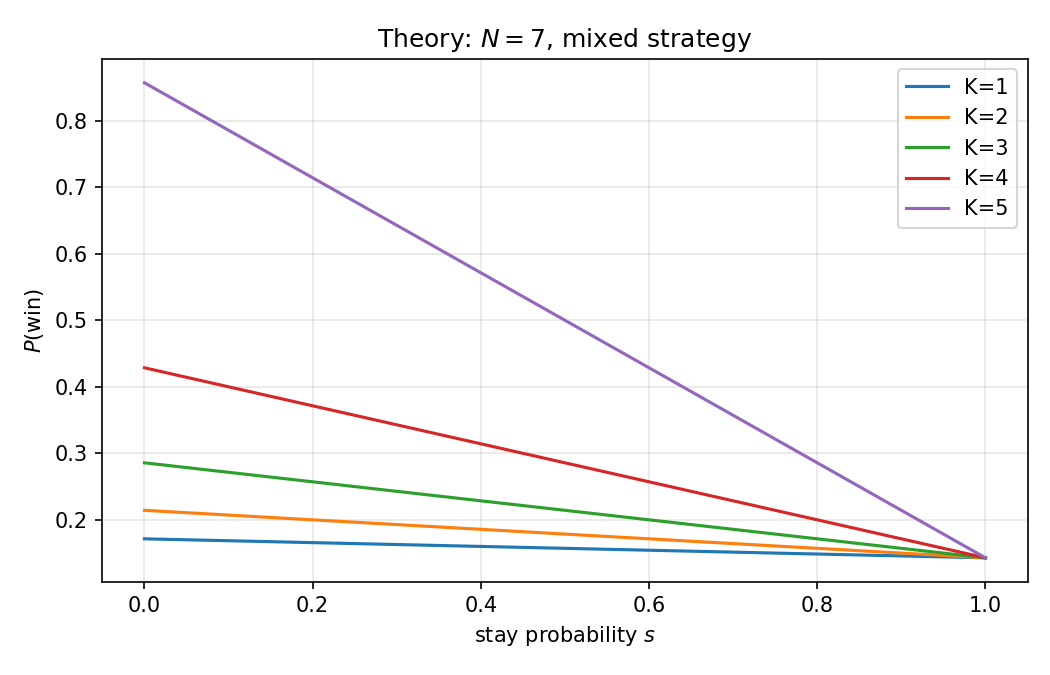
\includegraphics[width=0.92\textwidth]{hw2_prob_vs_switch.png}
\caption{Теоретическая $P(W)$ как функция $s$ при $N=7$ (подписи осей на графике на английском)}
\label{fig:pvs}
\end{figure}

\begin{figure}[H]
\centering
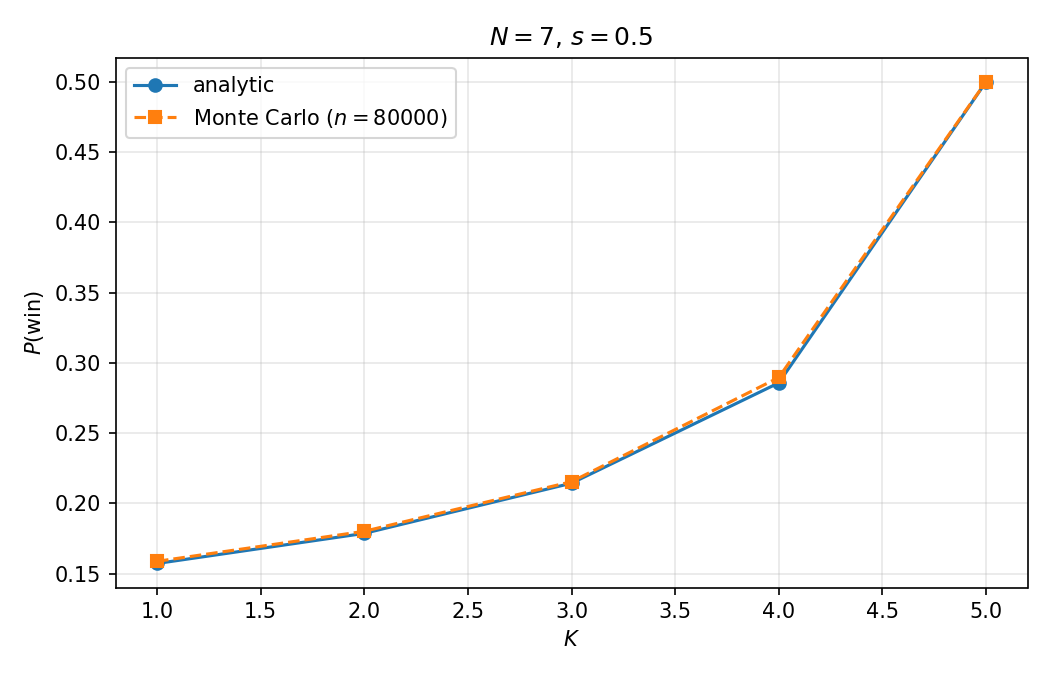
\includegraphics[width=0.92\textwidth]{hw2_theory_vs_mc_N7.png}
\caption{$N=7$, $s=0{,}5$: аналитика и Монте-Карло ($n=80000$ на каждое $K$; подписи на графике на английском)}
\label{fig:mc}
\end{figure}

\subsection{Варьирование числа прогонов $n$ при $N=7$, $K=3$, $s=0{,}5$}
Теоретически $p_{\text{теор}}=3/14 \approx 0{,}2143$. При малых $n$ оценка $\hat p$ может заметно отличаться от $p_{\text{теор}}$ из-за случайных флуктуаций; при росте $n$ отклонение в среднем уменьшается (см.~табл.~\ref{tab:sweep_n}).

\begin{table}[H]
\centering
\begin{tabular}{|c|c|c|c|}
\hline
$n$ & $\hat p$ & $p_{\text{теор}}$ & $| \hat p - p_{\text{теор}} |$ \\
\hline
10 & 0{,}10 & 0{,}2143 & 0{,}1143 \\
100 & 0{,}20 & 0{,}2143 & 0{,}0143 \\
1000 & 0{,}209 & 0{,}2143 & 0{,}0053 \\
10000 & 0{,}2148 & 0{,}2143 & 0{,}0005 \\
50000 & 0{,}2130 & 0{,}2143 & 0{,}0013 \\
100000 & 0{,}2159 & 0{,}2143 & 0{,}0016 \\
\hline
\end{tabular}
\caption{Согласованность оценки $\hat p$ с теорией в зависимости от объёма выборки (один и тот же \texttt{seed} в программе)}
\label{tab:sweep_n}
\end{table}

\subsection{Варьирование вероятности сохранения выбора $s$ при $N=7$, $K=3$, $n=50000$}
\begin{table}[H]
\centering
\begin{tabular}{|c|c|c|c|}
\hline
$s$ & $p_{\text{теор}}$ & $\hat p$ & $| \hat p - p_{\text{теор}} |$ \\
\hline
0 & 5/18 & 0{,}2891 & 0{,}0034 \\
0{,}25 & 1/4 & 0{,}2481 & 0{,}0019 \\
0{,}5 & 3/14 & 0{,}2130 & 0{,}0013 \\
0{,}75 & 5/28 & 0{,}1769 & 0{,}0017 \\
1 & 1/7 & 0{,}1429 & 0{,}0001 \\
\hline
\end{tabular}
\caption{Смешанная стратегия: разные соотношения «остаться --- сменить» при фиксированном $n$}
\label{tab:sweep_s}
\end{table}

\subsection{Полная сетка $(N,K)$ при $s=0{,}5$, $n=50000$}
{\footnotesize
\setlength{\LTleft}{\fill}
\setlength{\LTright}{\fill}
\begin{longtable}{|c|c|c|c|c|}
\hline
$N$ & $K$ & $p_{\text{теор}}$ & $p_{\text{МК}}$ & $|p_{\text{теор}}-p_{\text{МК}}|$ \\
\hline
\endfirsthead
\hline
$N$ & $K$ & $p_{\text{теор}}$ & $p_{\text{МК}}$ & $|\Delta|$ \\
\hline
\endhead
3 & 1 & 0{,}50000 & 0{,}49918 & 0{,}00082 \\
\hline
4 & 1 & 0{,}31250 & 0{,}31224 & 0{,}00026 \\
4 & 2 & 0{,}50000 & 0{,}49804 & 0{,}00196 \\
\hline
5 & 1 & 0{,}23333 & 0{,}22968 & 0{,}00365 \\
5 & 2 & 0{,}30000 & 0{,}30170 & 0{,}00170 \\
5 & 3 & 0{,}50000 & 0{,}49848 & 0{,}00152 \\
\hline
6 & 1 & 0{,}18750 & 0{,}18476 & 0{,}00274 \\
6 & 2 & 0{,}22222 & 0{,}22110 & 0{,}00112 \\
6 & 3 & 0{,}29167 & 0{,}29476 & 0{,}00309 \\
6 & 4 & 0{,}50000 & 0{,}49790 & 0{,}00210 \\
\hline
7 & 1 & 0{,}15714 & 0{,}15914 & 0{,}00200 \\
7 & 2 & 0{,}17857 & 0{,}17838 & 0{,}00019 \\
7 & 3 & 0{,}21429 & 0{,}21700 & 0{,}00271 \\
7 & 4 & 0{,}28571 & 0{,}28698 & 0{,}00127 \\
7 & 5 & 0{,}50000 & 0{,}50312 & 0{,}00312 \\
\hline
8 & 1 & 0{,}13542 & 0{,}13494 & 0{,}00048 \\
8 & 2 & 0{,}15000 & 0{,}15114 & 0{,}00114 \\
8 & 3 & 0{,}17188 & 0{,}16840 & 0{,}00348 \\
8 & 4 & 0{,}20833 & 0{,}21094 & 0{,}00261 \\
8 & 5 & 0{,}28125 & 0{,}27920 & 0{,}00205 \\
8 & 6 & 0{,}50000 & 0{,}49706 & 0{,}00294 \\
\hline
9 & 1 & 0{,}11905 & 0{,}11878 & 0{,}00027 \\
9 & 2 & 0{,}12963 & 0{,}12938 & 0{,}00025 \\
9 & 3 & 0{,}14444 & 0{,}14416 & 0{,}00028 \\
9 & 4 & 0{,}16667 & 0{,}16500 & 0{,}00167 \\
9 & 5 & 0{,}20370 & 0{,}20400 & 0{,}00030 \\
9 & 6 & 0{,}27778 & 0{,}27824 & 0{,}00046 \\
9 & 7 & 0{,}50000 & 0{,}50078 & 0{,}00078 \\
\hline
10 & 1 & 0{,}10625 & 0{,}10478 & 0{,}00147 \\
10 & 2 & 0{,}11429 & 0{,}11420 & 0{,}00009 \\
10 & 3 & 0{,}12500 & 0{,}12562 & 0{,}00062 \\
10 & 4 & 0{,}14000 & 0{,}14038 & 0{,}00038 \\
10 & 5 & 0{,}16250 & 0{,}16398 & 0{,}00148 \\
10 & 6 & 0{,}20000 & 0{,}19676 & 0{,}00324 \\
10 & 7 & 0{,}27500 & 0{,}27554 & 0{,}00054 \\
10 & 8 & 0{,}50000 & 0{,}50026 & 0{,}00026 \\
\hline
\end{longtable}
}

\section{Анализ модели и проверка качества}

После получения численных результатов необходимо проанализировать согласованность байесовской аналитики (формулы~\eqref{eq:bayes_posterior}, \eqref{eq:mixed}), программной реализации и данных Монте-Карло, а также проверить качество модели на граничных режимах.

\subsection{Анализ результатов сравнения теории и эксперимента}

\textbf{Классический случай ($N=3$, $K=1$).}
По табл.~\ref{tab:adequacy} оценки $\hat p$ для стратегий «остаться» и «сменить» близки к $p_{\text{теор}}$, вычисленным из~\eqref{eq:mixed}. При большом $n$ типичный масштаб случайной ошибки оценки $\hat p$ задаётся соотношением
\[
  \sigma_{\hat p} \approx \sqrt{\frac{p(1-p)}{n}}
\]
(частотная интерпретация: разброс выборочной доли при независимых повторениях). При $p\approx 1/3$ или $2/3$ и $n=200000$ величина $\sigma_{\hat p}$ порядка $10^{-3}$, что согласуется с наблюдаемыми $| \hat p - p_{\text{теор}} |$.

\textbf{Влияние объёма $n$ (табл.~\ref{tab:sweep_n}).}
При $n=10$ и $n=100$ отклонение $\hat p$ от $p_{\text{теор}}$ может быть заметным: для малых выборок одна и та же стохастическая модель даёт большой разброс частоты успехов. При $n \gtrsim 10^4$ оценка стабилизируется около $p_{\text{теор}}$; это согласуется с ожидаемым уменьшением $\sigma_{\hat p}$ при росте $n$.

\textbf{Влияние доли $s$ (табл.~\ref{tab:sweep_s}).}
При фиксированных $N$, $K$ величина $p_{\text{теор}}$ по~\eqref{eq:mixed} меняется линейно по $s$ между значениями~\eqref{eq:stay} и~\eqref{eq:switch}. Эксперимент при разных $s$ показывает, что симуляция воспроизводит эту линейную закономерность: наибольшие $| \hat p - p_{\text{теор}} |$ в таблице остаются в пределах нескольких тысячных при $n=50000$.

\textbf{Сетка $(N,K)$ при $s=0{,}5$.}
В длинной таблице раздела «Результаты» для каждой пары $(N,K)$ сопоставлены $p_{\text{теор}}$ по~\eqref{eq:mixed} и оценка $p_{\text{МК}}$ по $n=50000$ прогонов.
\begin{itemize}[nosep]
  \item Во всех $36$ ячейках сетки абсолютное отклонение $|\Delta| = |p_{\text{теор}} - p_{\text{МК}}|$ не превосходит $0{,}004$; для большинства пар оно меньше $0{,}003$.
  \item Наибольшие расхождения встречаются в отдельных точках (например, при малых $N$ и малых $K$), что соответствует большей относительной дисперсии $\hat p$ при малых $p_{\text{теор}}$ при том же $n$.
  \item При фиксированном $N$ и росте $K$ теоретическая вероятность~\eqref{eq:mixed} при $s=0{,}5$ монотонно возрастает от значений порядка $1/N$ до $1/2$ при $K=N-2$; кривые на рис.~\ref{fig:pvs} иллюстрируют аналогичную зависимость от $s$ для $N=7$.
  \item При $K=N-2$ и $s=0{,}5$ имеем $p_{\text{теор}}=1/2$; строки таблицы с $K=N-2$ показывают $p_{\text{МК}}$ около $0{,}5$.
\end{itemize}

\textbf{Графическое сопоставление.}
На рис.~\ref{fig:mc} для $N=7$, $s=0{,}5$ точки Монте-Карло лежат вблизи теоретической кривой по $K$ без систематического смещения.

\begin{table}[H]
\centering
\begin{tabular}{|l|c|}
\hline
\textbf{Показатель (полная сетка, $n=50000$)} & \textbf{Значение} \\
\hline
Число пар $(N,K)$ & $36$ \\
\hline
$\max |p_{\text{теор}} - p_{\text{МК}}|$ & $< 0{,}004$ \\
\hline
Типичный порядок $|\Delta|$ & $10^{-3}$ \\
\hline
\end{tabular}
\caption{Сводка отклонений аналитики и Монте-Карло на полной сетке}
\label{tab:grid_summary}
\end{table}

\subsection{Проверка качества модели}

\textbf{1. Соответствие постановке задачи.}
\begin{itemize}[nosep]
  \item Приз задаётся равновероятно по дверям; первый выбор игрока --- равновероятный.
  \item Ведущий открывает ровно $K$ пустых дверей среди допустимых; набор из $K$ дверей выбирается равновероятно --- в согласии с определением события $B$ и формулами $P(B\mid A)$, $P(B\mid \overline{A})$.
  \item На финальном шаге с вероятностью $s$ выбор сохраняется, с вероятностью $1-s$ --- переход к равновероятно выбранной другой закрытой двери.
  \item Логика симуляции согласована со схемой байесовской модели (рис.~\ref{fig:bayes_prob_tree}): сначала реализуются $A$/$\overline{A}$ и действие ведущего ($B$), затем --- финальное решение игрока.
\end{itemize}

\textbf{2. Граничные режимы.}
\begin{itemize}[nosep]
  \item $N=3$, $K=1$: см.~табл.~\ref{tab:adequacy}.
  \item $s=1$: $P(W)=1/N$; $s=0$: формула~\eqref{eq:switch}; при $K=N-2$ получается $P(W)=(N-1)/N$ при стратегии «сменить».
  \item Допустимые $K$ не выходят за пределы $1\le K\le N-2$.
\end{itemize}

\textbf{3. Ограничения.}
Модель не описывает произвольную (не равномерную) стратегию ведущего; при её изменении меняются $P(B\mid A)$, $P(B\mid \overline{A})$ и апостериорные вероятности.

\section{Выводы}

\begin{itemize}[nosep]
  \item Сформулирована байесовская модель через события $A$, $B$ и формулу~\eqref{eq:bayes_posterior}; получены явные выражения для $P(W)$ при стратегиях «остаться», «сменить» и смешанной стратегии~\eqref{eq:mixed}; определена стратегия Трикса ($s=0$).
  \item Реализована программная модель на Python; для $N=3$, $K=1$ частоты Монте-Карло согласуются с теоретическими $p_{\text{теор}}$ из той же постановки.
  \item Выполнено сравнение аналитики с Монте-Карло на сетке $N=3,\ldots,10$, $K=1,\ldots,N-2$ при $s=0{,}5$; дополнительно исследованы разные $s$ и объёмы $n$.
\end{itemize}

\end{document}
